%!TEX root = ../../dissertation.tex
%%%%%%%%%%%%%%%%%%%%%%%%%%%%%%%%%%%%%%%%%%%%%%%%%%%%%%%%%%%%%%%%%%%%%%%%%%%%%%%%
\section{Active Measurements and Testbeds}

Active measurements includes any kind of approach that generates its own network traffic and bases the evaluation on it. Therefore, they are usually conducted on an end-to-end base, with at lest one side under the control of the experimenter.

Apart from researchers writing their own specialized application for a singular study, active measurements are most often conducted with the help of existing network testbeds, thereby reducing the overall effort.
Any new or an alteration to existing network protocols are usually best tested in large-scale network testbeds to collect performance data and find side-effects. The presence of background traffic and a large device heterogeneity and diversity are often considered an advantage to a testbed as it better resembles real networks.

Testbeds can be either physically constructed by setting up a number of dedicated machines in a lab or form a virtual overlay spanning over an existing computer network. Both of these principles work well for wired network and there are a lot of examples of successful testbeds constructed with these principles.

Currently one of the largest installations is PlanetLab~\cite{chun2003planetlab}, consisting of dedicated machines located at a number of University sites. An experimenter can instantiate a \textit{slice} --- a portion of the overlay network made up of number of interconnected \glspl{VM} hosted on the various machines --- and conduct her studies. Thus, many experiments can run concurrently.

Several testbeds devote themselves to wireless and mobile networks. These are usually either put together in a clean lab environment, SmartLab\footnote{\url{http://smartlab.cs.ucy.ac.cy/}} or 
EmuLab\footnote{\url{http://www.emulab.net/}} come to mind, or hand out subsidized mobile devices prepared with custom firmwares to volunteers which need to allow running network experiments on them. The approach is taken, e.g., by NetSense~\cite{Striegel:2013:LLN:2491159.2491171} and PhoneLab\footnote{\url{https://www.phone-lab.org/}}~\cite{Nandugudi:2013:PLP:2536714.2536718}. The latter approach raises some interesting issues concerning the volunteers' privacy which will be covered in the next section.

All of these testbeds consist of rather uniform nodes and access to it still requires some amount of administrative effort, alternative approaches are also available, for example in the form of the Seattle Testbed\footnote{\url{https://seattle.poly.edu/html/}}~\cite{Cappos:2009:SPE:1508865.1508905}. Its overlay network comprises of small software sandboxes installable on a wide range of device types. Experimenters gain automatic access to a portion of the overlay through a clearing house and are resource-restricted to their slice by a hypervisor. As Seattle is available to both conventional PCs as well as Android smartphones, the overlay composition very heterogeneous. Therefore, the node stability and availability can vary substantially over time, caused amongst other things by the individual uptime of the computers following typical diurnal cycles and mobility-related connectivity issues.
While this forms a much more realistic picture of a network, it simultaneously makes the execution of the actual study more difficult as these churning issues have to be dealt with.

The requirements for conducting reliable streaming experiments are low. As it is usually a fully pull-based approach, full control over the server containing the streaming files is not necessary. It is also generally not necessary to display the actual video on the client in reliable streaming as it always will be a pixel-perfect representation. Therefore, the buffer-emulation measurement approach presented in \ref{c3:measurements} can be employed here. The measurement devices only have to record the transmission traces of the streaming process and make them available to the emulation process. The latter can for example also be performed in a centralized and asynchronous matter when dealing with non-adaptive streaming.


%%%%%%%%%%%%%%%%%%%%%%%%%%%%%%%%%%%%%%%%%%%%%%%%%%%%%%%%%%%%%%%%%%%%%%%%%%%%%%%%
\subsection{Enriching Mobile Measurements with Additional Metadata}
\label{c6:sensorium}

While transmission traces might be the bare minimum to conduct reliable streaming measurements, meaningful mobile measurement can include much more metadata, giving insightful indication of the device's current state.

Mobile devices have access to a vast array of data. On the one hand does the networking stack itself much information on its state, as discussed in the previous Chapter. The current radio and mobility state is especially relevant to mobile streaming measurements as it directly influences the link's \gls{QoS} parameters. 

But modern mobile devices additionally contain an ever-growing number of sensors, including \gls{GPS}, accelerometers, temperature, pressure, luminosity, humidity, fingerprint, heartbeat, and several cameras and microphones. Moreover, further radio interfaces (WiFi, Bluetooth, \acrshort{NFC}) gather data on network availability and signal quality. Each additional data source can help in quantifying the physical position, orientation and state of the device and even quantify the ``state'' of its user. Even the NSA is allegedly more interested in metadata in general than actual data for this reason.\footnote{\url{http://www.wired.com/2013/06/phew-it-was-just-metadata-not-think-again/}}

Active measurements in mobile networks should make use of metadata and correlate it to the regular measurement data to achieve a finer result granularity. Alternatively, sensor data can also be used for new kinds of evaluations. Questions like ``Can this device watch video at a an satisfactory quality at certain locations?'' can be raised and answered.


%%
\subsubsection{Metadata and Privacy}

While the actual experiment usually runs in a strict sandbox environment with no access to actual data on the device, allowing sensor and metadata access creates holes in the isolation model. As informative metadata can be for network studies as intrusive is unmediated access to this data for the device's user.

In a pure lab environment this poses no problem as there will be no device owner whose information can be leaked. However, preserving the privacy of actual device users running network testbed software is absolutely critical for a number of reasons:

\begin{itemize}

	\item For ethical reasons as stated in several ethics proclamations, for example in the well-known hacker ethics\footnote{\url{http://www.ccc.de/hackerethics}} which states to \textit{``Use public data, protect private data.''}. This is often called the principle of data economy and minimalization, aiming to prevent abuse and minimize the effects of accidental data leakage.

	\item User acceptance is a very important aspect. Testbeds need to have a sufficiently large installation base to achieve meaningful results. But users might choose not to participate if the testbed application is too intrusive. There needs to be a balance between revealing and protecting privacy sensitive data. The acceptance can also be increased by information and disclosing employed data. This servers the additional purpose of educating the user of privacy sensitive data.

	\item Lastly, there are legal constraints to consider when dealing with personal information. In Germany, for example, several fundamental constitutional rights restrict the use of personal data. These are the \textit{``Recht auf informationelle Selbstbestimmung''}\footnote{\url{https://www.bmi.bund.de/DE/Themen/Gesellschaft-Verfassung/Datenschutz/Informationelle-Selbstbestimmung/informationelle-selbstbestimmung_node.html}} and the \textit{``Grundrecht auf Gewährleistung der Vertraulichkeit und Integrität informationstechnischer Systeme''}\footnote{\url{https://www.bundesverfassungsgericht.de/entscheidungen/rs20080227_1bvr037007.html}}.

\end{itemize}

To conclude, network measurement testbeds have to regulate, filter, adjust, or outright prevent access to sensitive data. Existing testbeds usually do not take a technical but rather a bureaucratic approach to this problem. For example, all experiments in the aforementioned PhoneLab require approval from a review board.

But that does not mean, that there are no technical means available. Looking outside of the field of network testbeds, some research and even usable implementations are available.

A very basic and static approach to protecting privacy data is implemented in the regular versions of both iOS and Android. On installation any application has to request specific rights for each sensor source to be able to use it in the future. 
The ``Privacy Guard'' feature\footnote{\url{https://plus.google.com/+CyanogenMod/posts/gk7X3HjNvnH}} in the custom Android firmware CyanogenMod\footnote{\url{http://cyanogenmod.org/}} provides the additional capability to monitor and revoke any sensor permissions at runtime.

Other approaches include increasing the permission granularity~\cite{Jeon:2012:DAM:2381934.2381938} or tagging sensor data at the source to better track and find privacy leaks in Applications~\cite{enck2010taintdroid}.

%Improving wireless network performance using sensor hints \cite{ravindranath2011improving}


%%
\subsubsection{Preserving Testbed User Privacy with Sensorium}


%% ! <-- !
%%




no root rights required (e.g. compared to PhoneLab)
installable (apk, play, fdroid) on any Android device
can be metadata companion App to almost any smartphone-compatible testbed
leaves privacy choices with the user (decentralized)
drawback: experimenters have to cope with varying granularity of data
but: its real devices anyway, data will never be perfect, experiments always have to cope with this anyway
real people
guarantees through sandbox, not review boards

Sensorium play store stats:
usage peak: 51 concurrent device installs August 2014
total installs: 475 as of august 2014
on various types of devices (including tablets)
across several countries (top: US, DE, AT, India, Turkey)
and all carriers
with not particular advertisement (demo presentation at one national conference)



There exist problems for the practical viability of collection data though: Different devices and platforms such as Android and iOS use very different interfaces into their sensors; privacy is another issue hardly tackled on any platform other than in a crude binary (allow/deny access) way. Therefore, in this demo we introduce Sensorium, a generic sensor reading framework that funnels data from actual sensor drivers, implements fine-grained privacy control for the user, and provides generic outbound interfaces such as \acrshort{XML}-\acrshort{RPC}. We also show an application using it, \gls{O3GM}, which visualizes mobile coverage data coming from Sensorium.

%Sensor interfaces differ -> difficult to do generic stuff with them
Sensorium can access all the information a device provides and makes them available to other applications. Up until now, it has been a challenging task for software developers (especially scientists and experimenters) to implement specialized sensor applications. This task is simplified by providing a generic framework for interfacing sensors. In our current implementation, available for Android, most of the typical sensors are already implemented. Since giving access to sensor data also exposes the user's privacy, the user can disable or set privacy levels for each sensor individually, and all sensor readings that would be shared are displayed. %Setting higher privacy levels reduces the amount of data a sensor shares. %E.g., location data accuracy could be rounded, or just hashes of data shared.
\\

\gls{O3GM}\footnote{\url{https://o3gm.cs.univie.ac.at/o3gm/}} showcases the sensors framework. It comprises a web service displaying cellular access technology data points at their \gls{GPS} locations collected by devices running Sensorium (see Figure~\ref{c5:fig:ogggm}). This solves a real-world problem: Currently, this kind of data is only available to mobile operators, which however  are hindered by commercial interests to make them publicly available --- at least in raw, unadorned form. Other projects such as OpenSignalMaps\footnote{\url{http://opensignal.com/}} and Sensorly\footnote{\url{http://www.sensorly.com/}}, as well as corporations like Google and Apple collect these data, but are very restrictive regarding usage by other parties. This is not true for \gls{O3GM}: We make the data points collected available as Open Data under an open content license.

Obviously, other applications are possible. Since code and data are open-sourced, everyone can implement their great ideas, port Sensorium to other platforms or reimplement our interface there, etc.

\begin{figure}[htb]
\centering
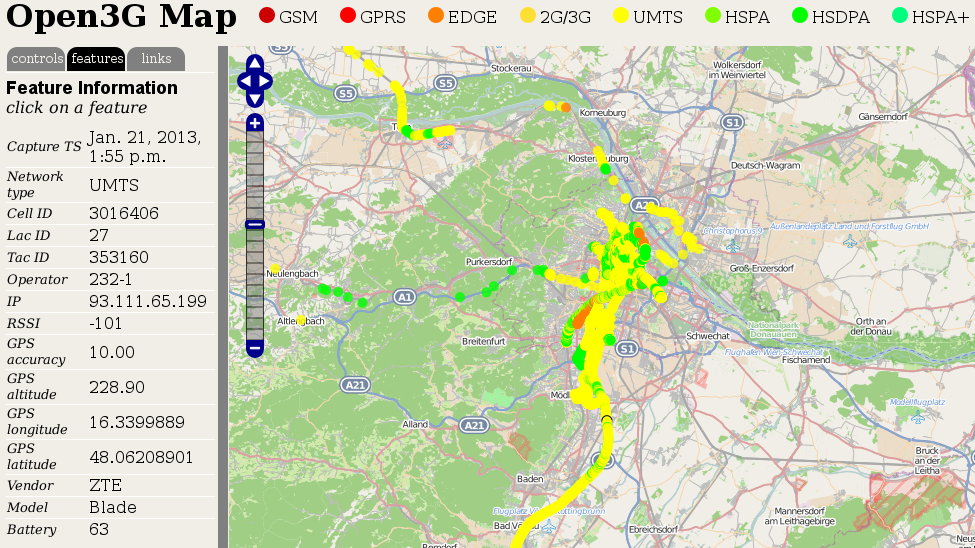
\includegraphics[width=\textwidth]{images/o3gm.png}
\caption{The \gls{O3GM} web page, displaying a \gls{3G} coverage measurements layer with data collected by Sensorium on top of the OpenStreetMap base layer.}
\label{c5:fig:ogggm}
\end{figure}

%\subsubsection{Architecture}

Figure~\ref{c5:fig:architecture} overviews Sensorium's architecture components, and its interplay with the data collecting parts of \gls{O3GM}. \textit{Sensor drivers} are implemented on top of the operating system taking care of reading sensor values from platform-specific interfaces and pushing them upwards into the \textit{registry}. Here, sensor data is timestamped and collected. On one side, data are prepared for local display, e.g., in a \gls{GUI} or status widget. On the other side, a user-configurable \textit{privacy layer} might allow for full sensor access from above or reduce the precision of values (e.g., round \gls{GPS} coordinates); it could salt and hash sensor values for improved privacy, or completely deny access to individual (or all) sensors. Finally, other applications running on the same device are free to connect to Sensorium's \textit{outbound interfaces} to register for sensor updates or poll data. Access from sources other than localhost is not allowed for obvious privacy reasons.

Due to the layered architecture, it is very simple for contributors to add their own implementations of layers or swap them out for their own altogether. Consider a scenario when a contributor wishes to include a sensor we do not yet provide a driver for. All that needs to be implemented is code interfacing the actual sensor, and the lightweight \gls{API} into our sensor registry. Similarly, additional local display methods, privacy enhancements, and outbound interfaces might be implemented.

\begin{figure}[htb]
	\centering
	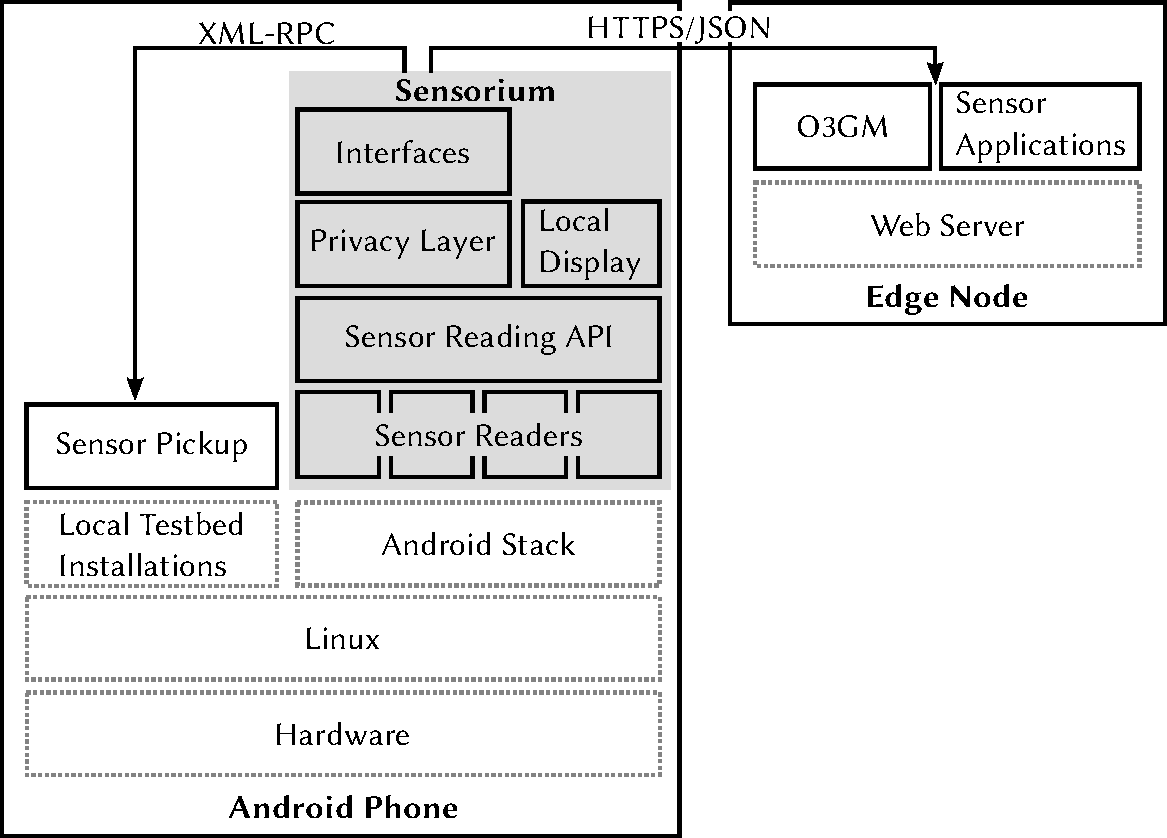
\includegraphics[width=0.8\textwidth]{images/sensorium-arch.pdf}
	\caption{Sensorium architecture with \gls{O3GM} \textit{pickup}~and \textit{server}. Previously existing components are marked with a dotted line.}
\label{c5:fig:architecture}
\end{figure}

%\subsubsection{Implementation}

Our current implementation of Sensorium\footnote{\url{https://github.com/fmetzger/android-sensorium}} runs on the Android platform. To provide a unified interface for accessing the sensor data we incorporated an \acrshort{XML}-\acrshort{RPC} library\footnote{\url{https://code.google.com/p/android-xmlrpc/}} that listens for connections on localhost, meaning that only applications running on the same device can access it. 
The pickup code to collect sensor values runs on top of the renowned Seattle\footnote{\url{https://seattle.poly.edu/html/}} platform, which is also available for Android, and allows us to remotely and securely access the collected data, and easily experiment with energy and cost efficient data upload/download strategies. 
The example application we implemented to make use of Sensorium, O3GM\footnote{\url{https://github.com/lukpueh/Open3GMap}}, is based on JavaScript and the OpenLayers\footnote{\url{http://openlayers.org/}} library. All of our code is dual-licensed under \gls{GPLv3} and the \acrshort{BSD} license.


\begin{figure}[htb]
        \centering
        \begin{subfigure}[b]{0.45\textwidth}
            \centering
			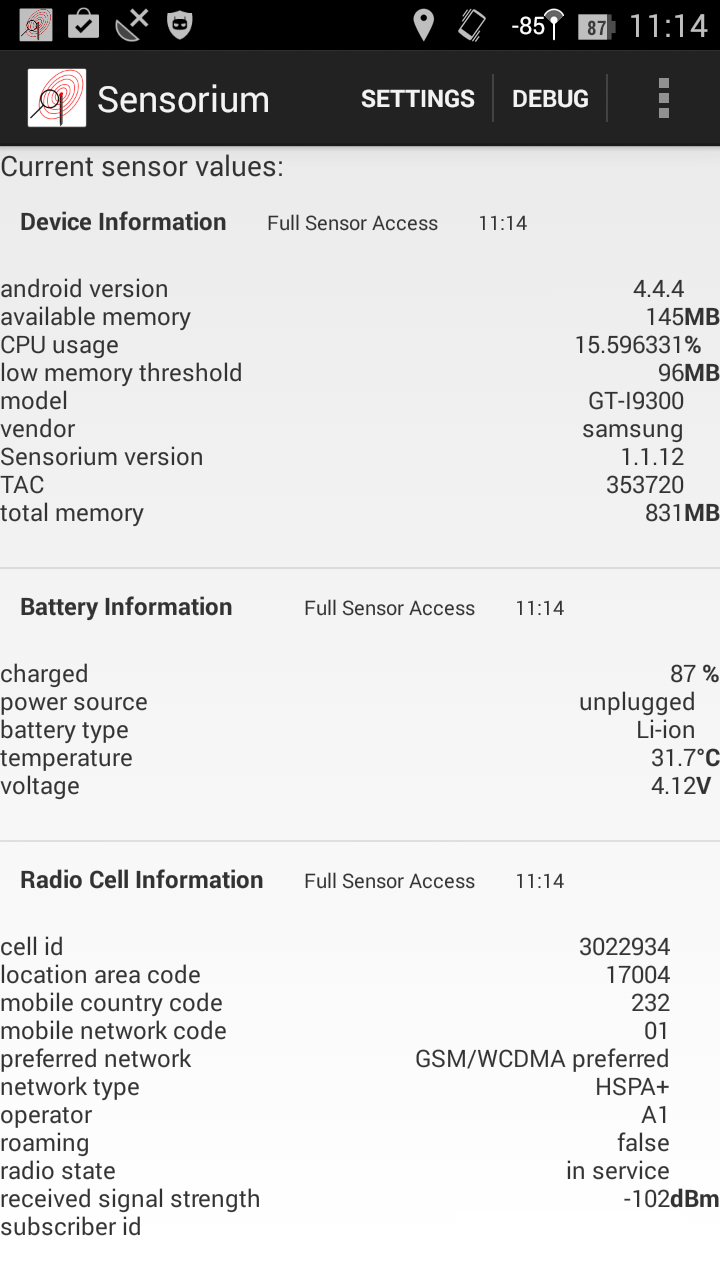
\includegraphics[width=\textwidth]{images/sensorium.png}
			%\caption{Stalling occurs without handover hinting.}
			%\label{c5:fig:streaming-hinting-no-cl}
        \end{subfigure}%
        \hfill
        \begin{subfigure}[b]{0.45\textwidth}
			\centering
			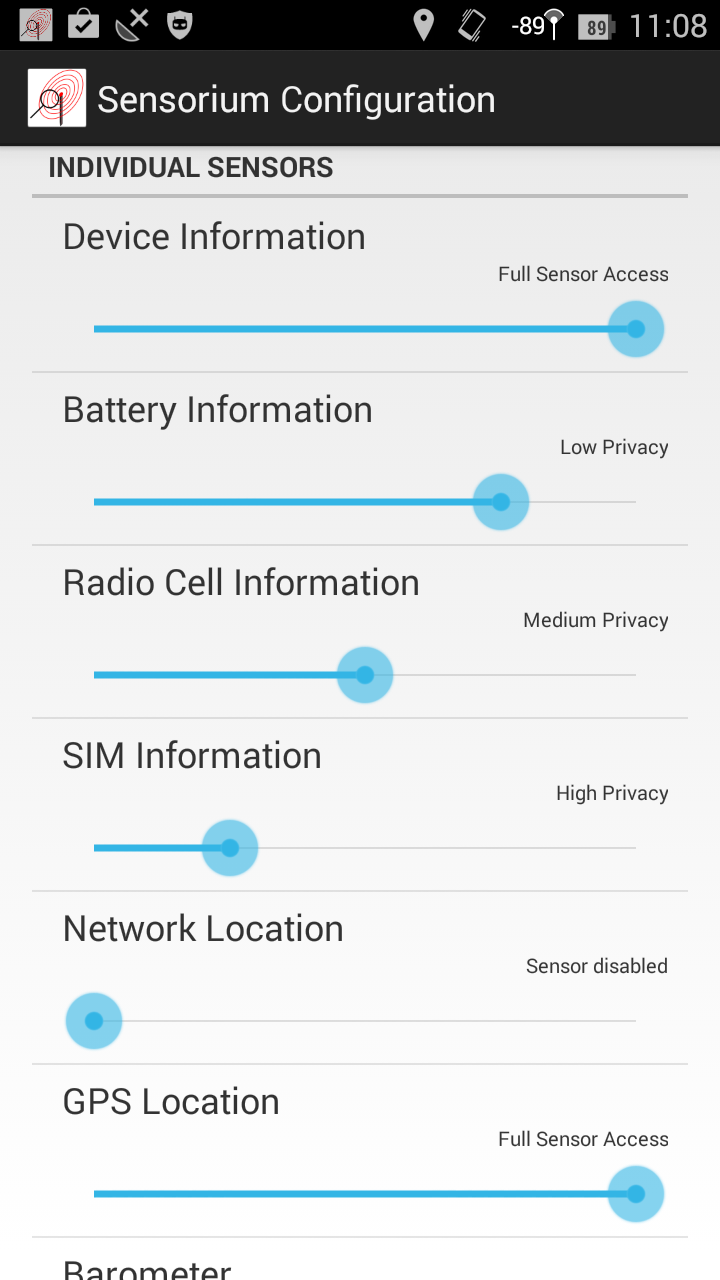
\includegraphics[width=\textwidth]{images/sensorium-settings.png}
			%\caption{Stalling can be prevented by hinting and proactively filling the playback buffer.}
			%\label{c5:fig:streaming-hinting-cl}
		   \end{subfigure}%
	\caption{Sensorium sensor values display and settings screenshots.}
\label{c5:fig:sensorium}
\end{figure}

Sensorium consists of a base registry service with a common interface which each sensor implementation can easily be plugged into. All values are also displayed for the user as seen in Figure~\ref{c5:fig:sensorium}. The privacy layer automatically anonymizes all gathered values before making them available through XML-RPC in accordance with the user's current privacy settings.

We currently provide sensor implementations for generic device information, e.g. device name and battery status; mobile radio data such as current access technology and cell information; location data provided by the mobile network and \gls{GPS}; and  WiFi and Bluetooth information, including recent scan results.

Sensorium attempts to bring the sensing capabilities of current generation devices to a broader range of developers and experimenters. Directly using Sensorium, which is freely available from the Google Play store, or adopting the available source code gives everyone the chance to build projects like the mobile coverage Web service we p
resented.


Follow-up: BlurSense\footnote{\url{https://blursense.poly.edu/projects/project}}~\cite{6798970}

Sensibility Testbed (https://sensibilitytestbed.com/projects/project): ``Followup''-Project to Sensorium, building entirely on Seattle/Python




% HomeLab: A Platform For Conducting Experiments With Connected Devices In The Home \cite{Singh:2013:HPC:2486001.2491701}
% authentication-based privacy, fully up to the experimenter

% phonelab privacy approach:
% Large (288 devices) smartphone testbed
% each participant can choose to participate in individual experiments
% open for experimenters upon approval, centralized experiment execution by the review board
% privacy guaranteed only through the project review board, not through technical means (centralized, not distributed)
% bureaucratic apprach to experimentation and privacy, not automatized
% relies on Androids privacy mechanisms (imho: do not work for this type of project)
% real people (as opposed to emulab, planetlab,...)!
% interesting study for wifi->3g vertical handover locations -> could extend wifi coverage studies and wifi planning

%http://campar.in.tum.de/Chair/KalmanFilter
%https://dsp.stackexchange.com/questions/320/is-a-kalman-filter-suitable-to-filter-projected-points-positions-given-euler-an/321\#321
%``Sensor Fusion''?

%https://guardianproject.info/

% NativeWrap \url{http://research.csc.ncsu.edu/security/nativewrap} \cite{Nadkarni:2014:NAH:2627393.2627412}
% Use website as app instead of native app, thus reducing permissions
